\documentclass[12pt,a4paper]{article}

% Packages
\usepackage[utf8]{inputenc}
\usepackage[margin=1in]{geometry}
\usepackage{fancyhdr}
\usepackage{graphicx}
\usepackage{amsmath}
\usepackage{hyperref}
\usepackage{titlesec}
\usepackage{enumitem}
\usepackage{tikz}
\usetikzlibrary{shapes,arrows,positioning}
\usepackage{xcolor}

% Define colors
\definecolor{sectioncolor}{RGB}{139,0,0}
\definecolor{subsectioncolor}{RGB}{220,20,60}

% Header and Footer Setup
\pagestyle{fancy}
\fancyhf{}
\fancyhead[L]{ROAR Solo Mission}
\fancyhead[R]{Part 1 Submission}
\fancyfoot[C]{\thepage}
\renewcommand{\headrulewidth}{0.4pt}
\renewcommand{\footrulewidth}{0.4pt}
\setlength{\headheight}{14.5pt}

% Prevent bad page breaks
\widowpenalty=10000
\clubpenalty=10000
\raggedbottom

% Title formatting
\titleformat{\section}
  {\normalfont\LARGE\bfseries\color{sectioncolor}}
  {\thesection}{1em}{}
  [\vspace{-0.5em}\textcolor{sectioncolor}{\titlerule[1.5pt]}\vspace{0.2em}]

\titleformat{\subsection}
  {\normalfont\Large\bfseries\color{subsectioncolor}}
  {\thesubsection}{1em}{}
  
\titlespacing*{\subsection}{0pt}{1em}{0.3em}
\titlespacing*{\section}{0pt}{1.5em}{0.5em}

\begin{document}

% Cover Page
\begin{titlepage}
    \centering
    \vspace*{2cm}
    
    {\Huge\bfseries ROAR Solo Mission}\\[0.5cm]
    {\LARGE Technical Documentation}\\[0.5cm]
    {\LARGE Part 1}\\[3cm]
    
    \vfill
    
    {\Large Prepared by:}\\[0.5cm]
    {\large Saif Elden Mahmoud}\\[3cm]
    
    {\Large Date:}\\[0.5cm]
    {\large \today}
    
    \vfill
    
\end{titlepage}

% Table of Contents
\tableofcontents
\newpage

% List of Figures
\listoffigures
\newpage

% Start of main content
\section{Autonomous Systems Fundamentals}

\subsection{Q1: What does it mean for a system to be autonomous?}

An autonomous system perceives its environment, processes information, and executes actions to achieve goals without continuous human intervention. Unlike automated systems that follow fixed rules, autonomous systems adapt to dynamic and unpredictable conditions.

\noindent\textbf{Core Architecture: Sense-Think-Act Loop}

The system operates through four interconnected modules:

\begin{enumerate}[leftmargin=*]
    \item \textbf{Perception} — Processes sensor data (LiDAR, cameras, RADAR) to detect and classify objects, producing an environmental map for planning.
    
    \item \textbf{Localization} — Determines the system's precise position and orientation by comparing sensor data against known maps and integrating motion data (GPS, IMU).
    
    \item \textbf{Planning} — The decision-making core that generates optimal trajectories using the environmental map and current position. Includes global route planning and local obstacle avoidance.
    
    \item \textbf{Control} — Translates planned trajectories into actuator commands (steering, throttle, braking) to execute the desired motion.
\end{enumerate}

\noindent\textbf{Data Flow:} Sensors $\rightarrow$ Perception \& Localization $\rightarrow$ Planning $\rightarrow$ Control $\rightarrow$ Actuators. This cycle repeats continuously at high frequency, enabling real-time adaptation.

\vspace{0.3em}
\noindent\rule{\textwidth}{0.4pt}
\vspace{0.3em}

\subsection{Q2: Role of simulation and testing}

Simulation and testing provide a continuous feedback loop that bridges conceptual design and safe physical deployment.


\begin{enumerate}[leftmargin=*]
    \item \textbf{System Design (Virtual Prototyping)} — Enables testing of different sensor configurations and algorithms without physical hardware costs. Design flaws are identified early through rapid software iteration.
    
    \item \textbf{Validation} — Two-stage verification process:
    \begin{itemize}
        \item \textit{Software-in-the-Loop (SIL):} Tests core logic in a purely virtual environment to verify correct code execution.
        \item \textit{Hardware-in-the-Loop (HIL):} Runs code on actual microcontrollers while simulating the physical world, validating real-time processing capabilities and communication protocols (CAN bus, I2C).
    \end{itemize}
    
    \item \textbf{Risk Reduction} — Safely tests dangerous edge cases (sensor failures, extreme weather, unexpected obstacles) that are impractical or unsafe to test physically. Automated regression testing ensures code updates don't break existing functionality.
\end{enumerate}

\vspace{0.3em}
\noindent\rule{\textwidth}{0.4pt}
\vspace{0.3em}

\subsection{Q3: Limitations of simulation environments}

Simulation cannot perfectly replicate reality due to the "Sim-to-Real" gap, caused by three technical discrepancies:

\begin{figure}[h]
\centering
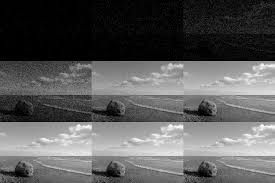
\includegraphics[width=0.7\textwidth]{Sensor Noise and Perception Artifacts.jpeg}
\caption{Sensor noise and perception artifacts in simulated vs. real environments}
\label{fig:sensor_noise}
\end{figure}

\begin{enumerate}[leftmargin=*]
    \item \textbf{Physics Simplification} — Simulators use idealized models for real-time performance:
    \begin{itemize}
        \item \textit{Non-linear Dynamics:} Real friction, tire slip, and aerodynamics vary with temperature and wear; simulators often use linear approximations.
        \item \textit{Deformable Objects:} Accurate modeling (e.g., tire deformation, cable flex) requires computationally expensive finite element analysis, typically omitted.
        \item \textit{Discrete Time Steps:} Physics calculated at intervals (e.g., 1ms) can miss fast collisions or become unstable, unlike continuous real-world physics.
    \end{itemize}
    
    \item \textbf{Sensor Noise and Perception Artifacts} — Simulated sensors are idealized unless explicitly degraded:
    \begin{itemize}
        \item \textit{Idealized Data:} Simulated LiDAR produces clean point clouds; real LiDAR suffers from multi-path reflections, ghosting in rain/fog, and infrared interference.
        \item \textit{Material Properties:} Simulators struggle with material-specific reflections (e.g., matte black surfaces may be invisible to real LiDAR but visible in simulation).
        \item \textit{Lens Effects:} Real cameras exhibit chromatic aberration and rolling shutter effects that are expensive to simulate accurately.
    \end{itemize}
    
    \item \textbf{Timing and Asynchronicity} — Simulators control time; reality does not:
    \begin{itemize}
        \item \textit{Jitter and Latency:} Simulated data exchange is instant; real systems have bus delays, contention, and electromagnetic interference causing stale data.
        \item \textit{Race Conditions:} Real hardware uses independent clocks, leading to dropped frames or delayed responses when sensors fire during CPU-intensive operations—scenarios synchronized simulations never encounter.
    \end{itemize}
\end{enumerate}

\subsection{Q4: What it means for a sensor model to be unrealistic}

In simulators like Gazebo, unrealistic sensor models provide "perfect" data that ignores physical and electrical imperfections of real hardware, creating a Sim-to-Real gap where systems perform flawlessly in simulation but fail in reality.

\begin{enumerate}[leftmargin=*]
    \item \textbf{Inaccurate Noise and Bias} — Simulators use simple Gaussian noise or none at all. Real sensors have bias (drifting constant offset) and non-linear noise. Control loops tuned for clean simulated data become unstable or jittery with real sensor signals.
    
    \item \textbf{Fixed vs. Variable Update Rates} — Simulators provide data at perfectly steady frequencies (e.g., exactly 50Hz). Real sensors experience latency and jitter from bus congestion (CAN, I2C). Timing-dependent algorithms (EKF, high-speed PID) fail when data arrives stale or irregularly.
    
    \item \textbf{Lack of Environmental Interaction} — Simulators treat surfaces as simple collision boxes. Real material properties matter: mirrors/windows may be invisible to LiDAR; dark carpets absorb IR beams. Perception modules fail to detect obstacles that were easily visible in simplified virtual environments.
    
    \item \textbf{Deterministic vs. Stochastic Behavior} — Simulators are deterministic (same input = same output). Real environments are stochastic with random interference (sunlight washing out cameras, electromagnetic interference from motors). Systems not stress-tested with random interference become fragile when deployed.
\end{enumerate}

\begin{figure}[h]
\centering
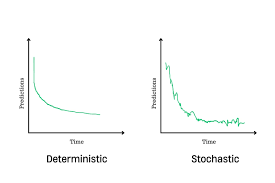
\includegraphics[width=0.65\textwidth]{Deterministic vs. Stochastic Behavior.png}
\caption{Deterministic simulation behavior vs. stochastic real-world conditions}
\label{fig:deterministic_stochastic}
\end{figure}

\section{ROS 2 Fundamentals}

\subsection{Q1: ROS 2 concepts}

In ROS 2, a robotic system is a collection of independent processes called Nodes that communicate using a Publish-Subscribe model.

\noindent\textbf{Core Components:}

\begin{itemize}[leftmargin=*]
    \item \textbf{Node} — Single-purpose executable (e.g., camera node, motor node).
    \item \textbf{Topic} — Named communication channel or "bus."
    \item \textbf{Message} — Data structure (e.g., Int32, Pose) sent over topics.
    \item \textbf{Publisher} — Node that sends data onto a topic.
    \item \textbf{Subscriber} — Node that listens for data on a topic.
    \item \textbf{Launch File} — Script (Python, XML, YAML) that starts multiple nodes with specific configurations.
\end{itemize}

\noindent\textbf{System Architecture Visualization:}

\begin{center}
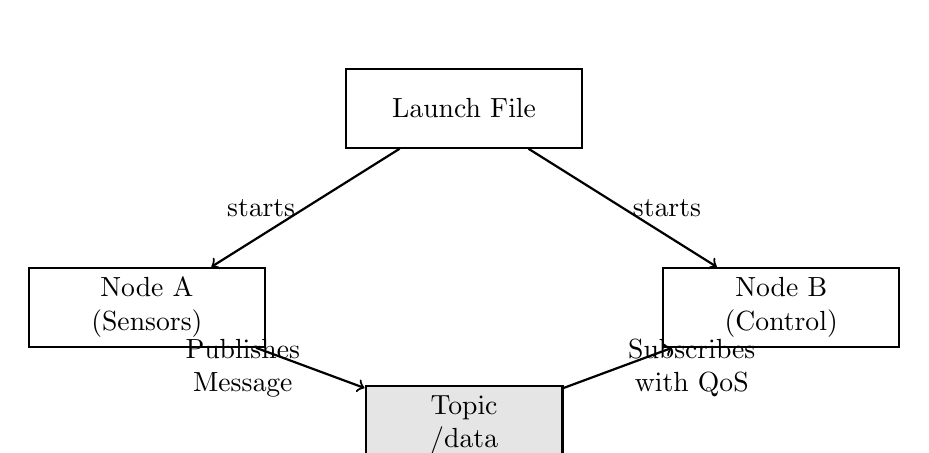
\begin{tikzpicture}[
    node distance=2cm,
    box/.style={rectangle, draw, thick, minimum width=3cm, minimum height=1cm, align=center},
    topic/.style={rectangle, draw, thick, fill=gray!20, minimum width=2.5cm, minimum height=0.8cm, align=center},
    arrow/.style={->, thick}
]
    % Launch File
    \node[box] (launch) {Launch File};
    
    % Node A
    \node[box, below left=1.5cm and 1cm of launch] (nodeA) {Node A\\(Sensors)};
    
    % Node B
    \node[box, below right=1.5cm and 1cm of launch] (nodeB) {Node B\\(Control)};
    
    % Topic
    \node[topic, below=3cm of launch] (topic) {Topic\\/data};
    
    % Arrows
    \draw[arrow] (launch) -- node[left, midway] {starts} (nodeA);
    \draw[arrow] (launch) -- node[right, midway] {starts} (nodeB);
    \draw[arrow] (nodeA) -- node[left, midway, align=center] {Publishes\\Message} (topic);
    \draw[arrow] (topic) -- node[right, midway, align=center] {Subscribes\\with QoS} (nodeB);
\end{tikzpicture}
\end{center}

\vspace{0.3em}
\noindent\rule{\textwidth}{0.4pt}
\vspace{0.3em}

\subsection{Q2: Quality of Service (QoS) Policies}

QoS policies tune node communication based on data requirements (e.g., "receive every packet" vs. "only latest data").

\noindent\textbf{Key Policies:}

\begin{enumerate}[leftmargin=*]
    \item \textbf{Reliability}
    \begin{itemize}
        \item \textit{Reliable:} Lost messages are resent (critical commands like emergency stop).
        \item \textit{Best Effort:} Messages sent once; losses are not recovered (high-frequency sensor data like LiDAR).
    \end{itemize}
    
    \item \textbf{Durability}
    \begin{itemize}
        \item \textit{Transient Local:} Publisher saves recent messages; late subscribers receive past messages (static data like map metadata).
        \item \textit{Volatile:} Late subscribers only see messages sent after connection.
    \end{itemize}
\end{enumerate}

\noindent\textbf{QoS Mismatch:} Connections form only if Publisher and Subscriber are compatible. The Subscriber must be at least as demanding as the Publisher.

\textit{Failure Scenario:} If Publisher uses Best Effort but Subscriber demands Reliable, the connection fails silently—the subscriber requires guarantees the publisher cannot provide, preventing message exchange.

\vspace{0.3em}
\noindent\rule{\textwidth}{0.4pt}
\vspace{0.3em}

\section{Path Planning}

\subsection{Q1: Path Planning Definition}

Path planning finds a geometric path from start to goal, bridging perception and action in the navigation stack. The robot must satisfy two constraint types:

\begin{itemize}[leftmargin=*]
    \item \textbf{Environmental Constraints} — Collision-free paths accounting for static and dynamic obstacles.
    \item \textbf{Kinematic Constraints} — Paths respecting physical limits (turning radius, maximum velocity). Example: car-like robots cannot move sideways.
\end{itemize}

\vspace{0.3em}
\noindent\rule{\textwidth}{0.4pt}
\vspace{0.3em}

\subsection{Q2: Global vs. Local Planners}

These planners work hierarchically to balance long-term goals with immediate safety:

\begin{itemize}[leftmargin=*]
    \item \textbf{Global Planner} — Operates on the entire known map to find the most efficient route. Uses static information (pre-loaded occupancy grid) and calculates infrequently.
    
    \item \textbf{Local Planner} — Focuses on a small window around the robot. Uses real-time sensor data (LiDAR, depth cameras) to detect dynamic obstacles and generates velocity commands.
\end{itemize}

\noindent\textbf{Interaction:} Global Planner provides waypoints; Local Planner follows them while avoiding obstacles not on the original map.

\vspace{0.3em}
\noindent\rule{\textwidth}{0.4pt}
\vspace{0.3em}

\subsection{Q3: Occupancy vs. Height Maps}

Environment representation depends on terrain complexity:

\begin{figure}[h]
\centering
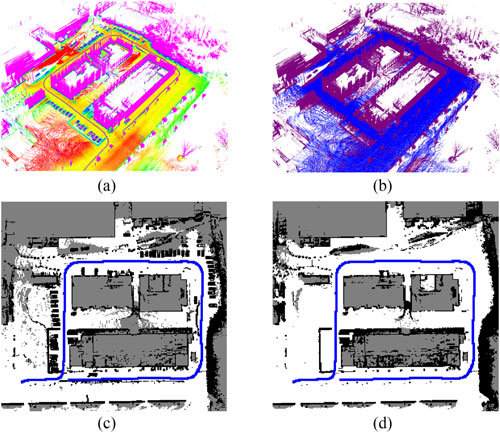
\includegraphics[width=0.7\textwidth]{Occupancy vs. Height Maps.jpeg}
\caption{Comparison of occupancy grid maps and height maps for terrain representation}
\label{fig:occupancy_height}
\end{figure}

\begin{itemize}[leftmargin=*]
    \item \textbf{Occupancy Grid Maps} — Discretize space into cells marked as "free," "occupied," or "unknown."
    \begin{itemize}
        \item \textit{Advantage:} Simple, memory-efficient for 2D navigation.
        \item \textit{Use Case:} Indoor mobile robots on flat floors.
    \end{itemize}
    
    \item \textbf{Height Maps (Elevation Maps)} — Store height (z) value for every (x,y) coordinate.
    \begin{itemize}
        \item \textit{Advantage:} Captures 3D geometry (slopes, curbs, steps) without full point cloud memory cost.
        \item \textit{Use Case:} Outdoor rovers or legged robots on uneven terrain.
    \end{itemize}
\end{itemize}

\vspace{0.3em}
\noindent\rule{\textwidth}{0.4pt}
\vspace{0.3em}

\subsection{Q4: A* Algorithm}

A* is a heuristic-based search algorithm that finds the least-cost path by evaluating nodes using:

$$f(n) = g(n) + h(n)$$

Where:
\begin{itemize}[leftmargin=*]
    \item $g(n)$ — Actual cost from start node to current node $n$
    \item $h(n)$ — Heuristic estimate of cost from $n$ to goal (e.g., Euclidean distance)
\end{itemize}

\noindent\textbf{Optimality Guarantee:} A* finds the optimal path if the heuristic is:
\begin{itemize}[leftmargin=*]
    \item \textit{Admissible:} Never overestimates true cost to goal
    \item \textit{Consistent:} Satisfies triangle inequality
\end{itemize}

\noindent\textbf{Comparison with Dijkstra's:} Dijkstra's is A* with $h(n) = 0$. It explores all directions equally (breadth-first), always finding the shortest path but much slower than A* because it lacks directional guidance toward the goal.

\vspace{0.3em}
\noindent\rule{\textwidth}{0.4pt}
\vspace{0.3em}

\subsection{Q5: Artificial Potential Field (APF)}

APF treats the robot as a particle in a virtual magnetic field, moving according to the gradient of a potential function combining two forces:

\begin{figure}[h]
\centering
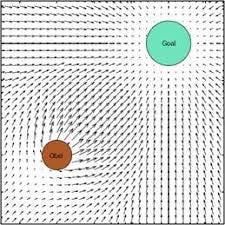
\includegraphics[width=0.65\textwidth]{Artificial Potential Field.jpg}
\caption{Artificial Potential Field concept showing attractive and repulsive forces}
\label{fig:apf}
\end{figure}

\begin{itemize}[leftmargin=*]
    \item \textbf{Attractive Force ($F_{att}$)} — Pulls robot toward goal; strength increases with distance from target.
    \item \textbf{Repulsive Force ($F_{rep}$)} — Pushes robot away from obstacles; very strong when close, drops to zero outside safety buffer.
\end{itemize}

The robot follows the resultant force: $F_{total} = F_{att} + F_{rep}$, sliding down the potential gradient toward the goal.

\noindent\textbf{Mathematical Formulation:}

Total potential field: $U(q) = U_{att}(q) + U_{rep}(q)$

Resulting force: $F(q) = -\nabla U(q)$

Where $U_{att}$ is typically quadratic: $\frac{1}{2}\xi\rho^2(q, q_{goal})$, and $U_{rep}$ is inversely proportional to obstacle distance.

\noindent\textbf{Main Limitations:}

\begin{enumerate}[leftmargin=*]
    \item \textbf{Local Minima} — Forces cancel before reaching goal (e.g., U-shaped obstacles), causing robot to get stuck.
    \item \textbf{Oscillations} — Rapid bouncing between repulsive forces in narrow passages leads to unstable movement.
    \item \textbf{GNRON (Goal Non-Reachable with Obstacles Nearby)} — Obstacles very close to goal prevent robot from reaching target due to strong repulsive forces.
\end{enumerate}

\vspace{0.3em}
\noindent\rule{\textwidth}{0.4pt}
\vspace{0.3em}

\section{Control}

\subsection{Q1: Define Control Theory}

Control theory provides the mathematical framework that translates high-level commands ("go there") into precise actuator signals ("send 3.3V to steering motor").

\begin{figure}[h]
\centering
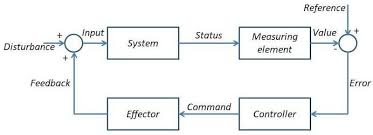
\includegraphics[width=0.7\textwidth]{Define Control Theory.jpeg}
\caption{Control theory framework translating commands to actuator signals}
\label{fig:control_theory}
\end{figure}

\noindent\textbf{Purpose:} Manages physical system behavior to execute commands smoothly and accurately.

\noindent\textbf{Challenge:} Forces hardware to follow software commands while actively compensating for real-world physics (momentum, friction, wind resistance, sensor noise).

\noindent\textbf{Key Components:}
\begin{itemize}[leftmargin=*]
    \item \textit{Plant:} The physical system being controlled (vehicle, robot arm)
    \item \textit{Controller:} Algorithm computing control signals
    \item \textit{Actuators:} Hardware executing commands (motors, servos)
    \item \textit{Sensors:} Measuring system state for feedback
\end{itemize}

\vspace{0.3em}
\noindent\rule{\textwidth}{0.4pt}
\vspace{0.3em}

\subsection{Q2: Open-loop vs. Closed-loop Control}

The fundamental distinction: checking your work versus hoping for the best.

\begin{figure}[h]
\centering
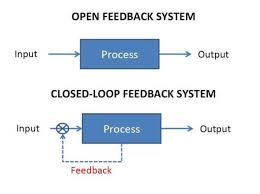
\includegraphics[width=0.75\textwidth]{Open-loop vs. Closed-loop Control.jpeg}
\caption{Open-loop control (blind) vs. closed-loop control (feedback-based)}
\label{fig:open_closed_loop}
\end{figure}

\begin{itemize}[leftmargin=*]
    \item \textbf{Open-loop (Blind)} — Sends command without verification (e.g., "spin tires for 3 seconds"). If vehicle slips on ice, system remains unaware it didn't move. Simple but unreliable in unpredictable environments.
    
    \item \textbf{Closed-loop (Aware)} — Uses sensor feedback to continuously measure error (desired state - actual state) and adjust control signals. Robust to disturbances but requires accurate sensors and careful tuning.
\end{itemize}

\noindent\textbf{Example:} Open-loop cruise control maintains fixed throttle; closed-loop adjusts throttle based on actual speed measurement.

\vspace{0.3em}
\noindent\rule{\textwidth}{0.4pt}
\vspace{0.3em}

\subsection{Q3: Controller Stability}

Stability determines whether a system behaves predictably or catastrophically.

\begin{figure}[h]
\centering
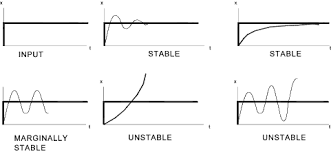
\includegraphics[width=0.7\textwidth]{Controller Stability.png}
\caption{Stable vs. unstable controller behavior over time}
\label{fig:controller_stability}
\end{figure}

\begin{itemize}[leftmargin=*]
    \item \textbf{Stable Behavior} — System returns to desired state after disturbances. If wind pushes vehicle off course, controller gently steers back without overshooting.
    
    \item \textbf{Unstable Behavior} — System overreacts to errors, causing oscillations that grow over time. Small steering error triggers excessive correction, leading to violent swerving and potential crash.
\end{itemize}

\noindent\textbf{Mathematical Criterion:} A system is stable if all poles of its transfer function have negative real parts (for continuous systems) or magnitude less than 1 (for discrete systems).

\vspace{0.3em}
\noindent\rule{\textwidth}{0.4pt}
\vspace{0.3em}

\subsection{Q4: Pure Pursuit Algorithm}

Pure Pursuit mimics how a dog chases a rabbit—aiming for where the target will be, not where it is.

\begin{figure}[h]
\centering
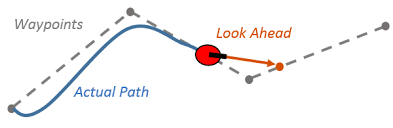
\includegraphics[width=0.7\textwidth]{Pure Pursuit Algorithm.png}
\caption{Pure Pursuit algorithm geometry showing lookahead point and circular arc}
\label{fig:pure_pursuit}
\end{figure}

\noindent\textbf{Concept:} Algorithm selects a "lookahead point" at fixed distance ahead on desired path.

\noindent\textbf{Geometry:} Calculates circular arc connecting vehicle's rear axle to lookahead point. The arc radius determines required steering angle.

\noindent\textbf{Output:} Steering command: $\delta = \arctan\left(\frac{2L\sin(\alpha)}{l_d}\right)$

Where $L$ is wheelbase, $\alpha$ is angle to lookahead point, $l_d$ is lookahead distance.

\noindent\textbf{Advantage:} Geometrically simple, computationally efficient, naturally smooth trajectories.

\vspace{0.3em}
\noindent\rule{\textwidth}{0.4pt}
\vspace{0.3em}

\subsection{Q5: Standard vs. Adaptive Pure Pursuit}

Lookahead distance dramatically affects performance at different speeds.

\begin{figure}[h]
\centering
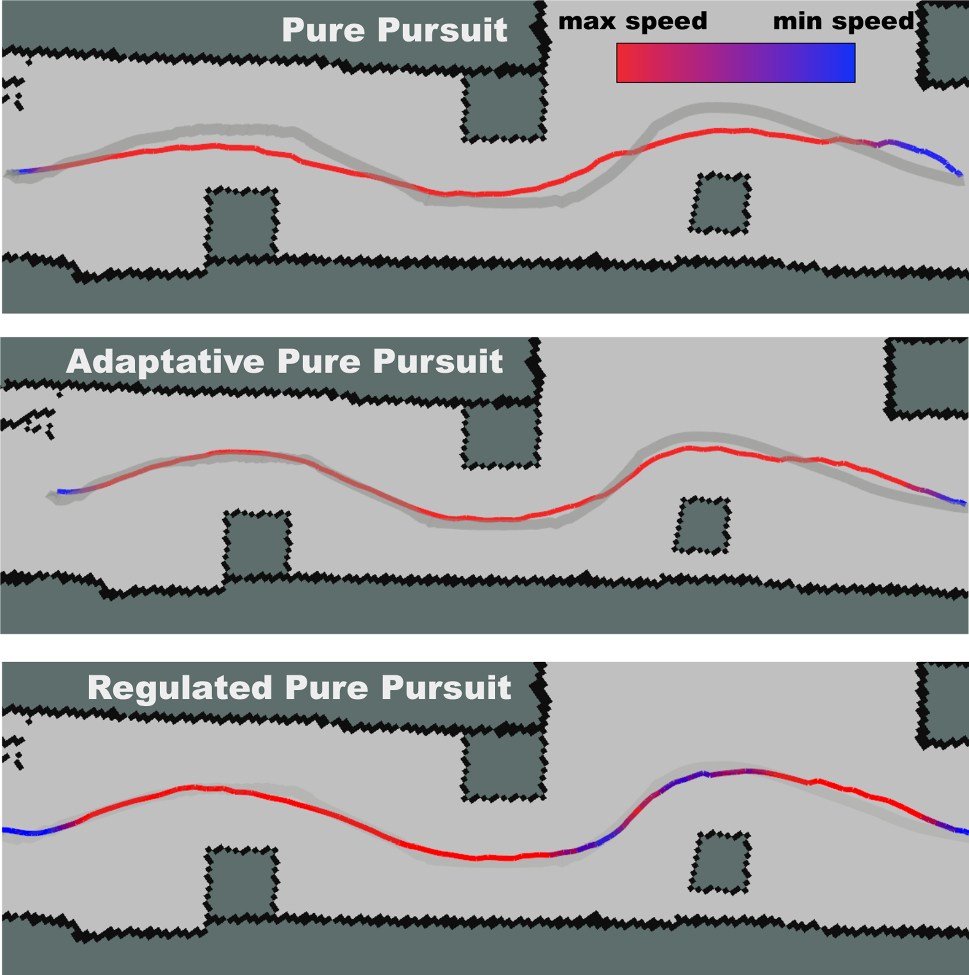
\includegraphics[width=0.7\textwidth]{adaptive pure pursuit.png}
\caption{Adaptive Pure Pursuit adjusting lookahead distance based on velocity}
\label{fig:adaptive_pursuit}
\end{figure}

\begin{itemize}[leftmargin=*]
    \item \textbf{Standard Pure Pursuit} — Fixed lookahead distance. Optimal at one speed but problematic at others. Short distance at high speed causes aggressive swerving; long distance at low speed results in wide corner cutting.
    
    \item \textbf{Adaptive Pure Pursuit} — Dynamically adjusts lookahead: $l_d = k_v \cdot v + l_{min}$, where $k_v$ is velocity gain and $l_{min}$ is minimum distance. Stretches lookahead at high speeds (smooth lane changes) and shrinks at low speeds (tight cornering).
\end{itemize}

\noindent\textbf{Benefit:} Prevents high-speed instability while maintaining low-speed precision, adapting to vehicle dynamics across operating range.

\vspace{0.3em}
\noindent\rule{\textwidth}{0.4pt}
\vspace{0.3em}

\section{Localization}

\subsection{Q1: Sensor Fusion Concept}

Sensor fusion mathematically blends data from multiple sensors to create a single, highly accurate world representation—like a team where each member has unique strengths covering others' weaknesses.

\noindent\textbf{Why Necessary:} No single sensor is perfect:
\begin{itemize}[leftmargin=*]
    \item \textit{Cameras:} Excellent for lane detection but blind at night or in direct sunlight
    \item \textit{LiDAR:} Performs well in darkness but confused by rain or fog
    \item \textit{GPS:} Provides global position but fails in tunnels or urban canyons
\end{itemize}

\noindent\textbf{Result:} When one sensor fails or becomes noisy, others compensate instantly, preventing system failure. Fusion algorithms weight sensor contributions based on current reliability, creating robust state estimates.

\vspace{0.3em}
\noindent\rule{\textwidth}{0.4pt}
\vspace{0.3em}

\subsection{Q2: IMU and Drift}

An Inertial Measurement Unit (IMU) measures motion without external references—like closing your eyes in a moving car and sensing acceleration and turns.

\noindent\textbf{Structure:} Packages three sensors on one chip:
\begin{itemize}[leftmargin=*]
    \item \textit{Accelerometer:} Measures linear forces and gravity
    \item \textit{Gyroscope:} Measures rotation rates
    \item \textit{Magnetometer:} Digital compass (optional)
\end{itemize}

\noindent\textbf{Role in Localization:} GPS updates slowly ($\sim$10 Hz); IMU provides high-frequency updates (100+ Hz) to estimate pose between GPS measurements.

\noindent\textbf{The Flaw (Drift):} Position requires double integration of acceleration. Sensor noise, though small, accumulates rapidly through integration. After seconds, drift occurs—the system believes it moved meters while actually stationary. Fusion with absolute position sensors (GPS, visual landmarks) corrects this drift.

\vspace{0.3em}
\noindent\rule{\textwidth}{0.4pt}
\vspace{0.3em}

\subsection{Q3: Kalman vs. Extended Kalman Filter}

These algorithms balance model predictions with noisy sensor measurements—the ultimate "trust but verify" approach.

\begin{itemize}[leftmargin=*]
    \item \textbf{Standard Kalman Filter (KF)} — Optimal for linear systems where relationships scale in straight lines.
    \begin{itemize}
        \item \textit{How it works:} Recursively estimates true state by minimizing mean squared error
        \item \textit{When to use:} Simple 1D problems (temperature tracking, straight-line motion)
        \item \textit{Limitation:} Assumes linear dynamics and measurement models
    \end{itemize}
    
    \item \textbf{Extended Kalman Filter (EKF)} — Handles non-linear systems using linearization.
    \begin{itemize}
        \item \textit{How it works:} Uses Jacobian matrices (calculus) to locally linearize non-linear functions (sine, cosine in rotation) at each time step
        \item \textit{When to use:} Modern robotics with steering, rotation, and multiple sensors
        \item \textit{Advantage:} Handles realistic vehicle dynamics (turning arcs, sensor rotations)
    \end{itemize}
\end{itemize}

\noindent\textbf{Key Difference:} KF assumes $x_{k+1} = Ax_k + Bu_k$; EKF linearizes $x_{k+1} = f(x_k, u_k)$ using $\frac{\partial f}{\partial x}$.

\vspace{0.3em}
\noindent\rule{\textwidth}{0.4pt}
\vspace{0.3em}

\section{Perception}

\subsection{Q1: LiDAR vs. Cameras}

The fundamental difference: feeling your way with a precise tape measure versus looking around with your eyes.

\begin{figure}[h]
\centering
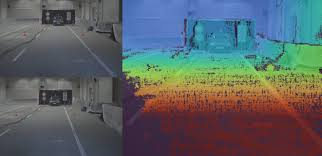
\includegraphics[width=0.75\textwidth]{lidar vs camera.jpeg}
\caption{LiDAR (active sensing) vs. Camera (passive sensing) comparison}
\label{fig:lidar_camera}
\end{figure}

\noindent\textbf{How They Work:}
\begin{itemize}[leftmargin=*]
    \item \textbf{LiDAR (Active)} — Emits millions of laser pulses per second, measuring Time-of-Flight (how long light takes to bounce back).
    \item \textbf{Camera (Passive)} — Captures ambient light (photons) bouncing off objects onto its image sensor.
\end{itemize}

\noindent\textbf{Data Output:}
\begin{itemize}[leftmargin=*]
    \item \textit{LiDAR:} 3D Point Cloud with exact (X, Y, Z) coordinates. Inherently knows distance but is colorblind.
    \item \textit{Camera:} 2D Pixel Grid (RGB image). Knows color and texture but has no native depth information.
\end{itemize}

\noindent\textbf{Processing Requirements:}
\begin{itemize}[leftmargin=*]
    \item \textit{LiDAR:} Low processing load for obstacle detection. Simple rule-based logic: "if point $<$ 1m, brake."
    \item \textit{Camera:} High processing load. Requires heavy AI/Neural Networks to distinguish pedestrians from painted signs.
\end{itemize}

\noindent\textbf{Failure Conditions:}
\begin{itemize}[leftmargin=*]
    \item \textit{LiDAR:} Laser scatter in heavy rain, fog, snow, or reflective surfaces (glass, mirrors).
    \item \textit{Camera:} Poor lighting—pitch black, blinding sunlight glare, rapid transitions (tunnel exit).
\end{itemize}

\vspace{0.3em}
\noindent\rule{\textwidth}{0.4pt}
\vspace{0.3em}

\subsection{Q2: Monocular vs. Stereo Cameras}

The difference between covering one eye versus using both.

\begin{figure}[h]
\centering
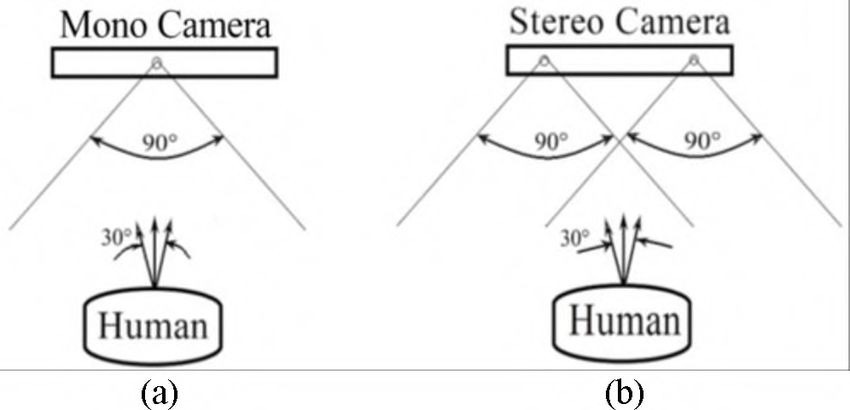
\includegraphics[width=0.7\textwidth]{Mono vs Stero camera.png}
\caption{Monocular (single) vs. Stereo (dual) camera depth estimation}
\label{fig:mono_stereo}
\end{figure}

\begin{itemize}[leftmargin=*]
    \item \textbf{Monocular (Single Camera)}
    \begin{itemize}
        \item \textit{Depth Estimation:} No native depth perception. Uses contextual tricks—if a known 75cm stop sign appears small, AI infers it's far away.
        \item \textit{Complexity:} Computationally cheap, inexpensive hardware. Easily runs on Raspberry Pi.
        \item \textit{Limitation:} Depth estimates are unreliable for unknown objects.
    \end{itemize}
    
    \item \textbf{Stereo (Dual Cameras)}
    \begin{itemize}
        \item \textit{Depth Estimation:} Works like human eyes. Views same object from two angles, measures horizontal disparity (pixel shift between left/right images) to calculate exact distance.
        \item \textit{Complexity:} Computationally heavy. Must process two HD streams, match corresponding pixels in real-time, and compute depth for every pixel.
        \item \textit{Advantage:} Accurate depth for any object, not just known ones.
    \end{itemize}
\end{itemize}

\noindent\textbf{Mathematical Basis:} Stereo depth: $Z = \frac{f \cdot B}{d}$, where $f$ is focal length, $B$ is baseline (camera separation), $d$ is disparity.

\vspace{0.3em}
\noindent\rule{\textwidth}{0.4pt}
\vspace{0.3em}

\subsection{Q3: ArUco Markers}

Simplified, ruggedized QR codes designed for robotic vision—readable from across a room.

\begin{figure}[h]
\centering
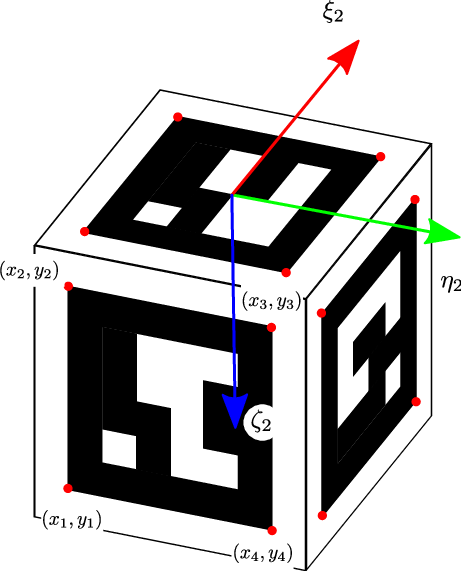
\includegraphics[width=0.65\textwidth]{ArUco.png}
\caption{ArUco marker detection and 6D pose estimation for robotic applications}
\label{fig:aruco}
\end{figure}

\noindent\textbf{Structure \& Detection:} High-contrast black-and-white square grids. Camera algorithm converts image to grayscale, detects stark black square outlines, extracts inner binary pattern, and matches against known dictionary to identify valid markers.

\noindent\textbf{Information Extracted:}
\begin{itemize}[leftmargin=*]
    \item \textit{Marker ID:} Identifies which specific marker (e.g., "Marker \#42")
    \item \textit{6D Pose:} Calculates position (X, Y, Z) and orientation (Roll, Pitch, Yaw). Since markers are perfect flat squares, any skewed trapezoid appearance reveals exact 3D pose through perspective geometry.
\end{itemize}

\noindent\textbf{Applications:}
\begin{enumerate}[leftmargin=*]
    \item \textbf{Localization} — Place Marker \#1 on a wall. When rover detects it, instantly calculates its exact room position relative to the wall.
    \item \textbf{Manipulation} — Attach marker to tool or box. Robotic arm uses 6D pose to angle gripper perfectly for precise grasping.
\end{enumerate}

\noindent\textbf{Advantage:} Provides absolute position reference without GPS, enabling precise indoor navigation and object manipulation.

\end{document}
